\chapter{Count Models}\label{chap:count-models}
So-called \emph{count models} were the first methods investigated for creating word embeddings. They emerged from work in the field of information retrieval (IR). In particular, influential contributions \parencite{dublin-2004-the-most-influential} were made by \citeauthor{salton-1975-a-vector-space-model}'s \parencite*{salton-1975-a-vector-space-model} work on the SMART information retrieval system which ``pionered many of the concepts that are used in modern search engines'' \parencite{turney10-from-frequen-to-meanin}. Initally word-similarity was not the focus of the developed models, but instead \emph{document similarity} was (for matching search queries to relevant/related material), however \textcite{deerwester-1990-indexing-by-lsa} observed that by looking at row vectors rather than column vectors in a document-term matrix the objects described were \emph{word vectors}.


Co-occurrence matricies, the heart of \emph{count models} do what they say: they count instances of co-occurrence. They can be thought of like big tally tables.

We use the framework described by \textcite{turney10-from-frequen-to-meanin} to group ``count models'' according to the structure (choice of rows and columns) of the co-occurence matrix they create. In the case of document-term matricies which we discuss first, the rows represent documents and the columns represent terms in the vocabulary of the document corpus. In the case of word-context matricies the rows represent target words (occuring at the center of a context-window), and the columns represent context words (occuring in a target word's context-window).

\section{Document-term Matricies}
\begin{definition}[Document-term co-occurrence count]
  In the context of document-term matricies, the function $f(w,W_d)$ indicates the number of times the token $w$ appears in a tokenized document $W_d$.
\end{definition}

\begin{definition}[Document-term matricies]
  Given a corpus of documents $C=d_1,d_2,\dots,d_n$, and a tokenizer $T$, a term document matrix $\bf{X}$ is given by:
  \begin{equation}
    \bf{X}=
  \begin{bmatrix}
    f(w_1, W_{d_1}) & f(w_1, W_{d_2}) & \dots  & f(w_1, W_{d_n}) \\
    f(w_2, W_{d_1}) & f(w_2, W_{d_2}) & \dots  & f(w_2, W_{d_n}) \\
    \vdots        & \vdots        & \ddots & \vdots          \\
    f(w_m, W_{d_1}) & f(w_m, W_{d_2}) & \dots  & f(w_m, W_{d_n}) \\
  \end{bmatrix}
  \end{equation}
  where the $w_i$ terms are from the vocabulary of $C$, $V(C)=w_1,w_2,\dots,w_m$.
  The number of times the $i^{\text{th}}$ word appears in the $j^{\text{th}}$ document then, is given by $\bf{X}_{ij}$.
\end{definition}

\begin{example}[Plato Document Vectors]
  A document-term co-occurrence matrix has document-vectors for columns and word-vectors for rows. Here we present a section of a document-term matrix for the tokenized Plato corpus, and show in \autoref{fig:plato-docs} how these counts can be used to position document-vectors in a term-space.
  \begin{center}
  \captionsetup{width=.91\linewidth}
    \begin{tabular}{c r r r r r r}
      \toprule
      {\multicolumn{1}{c}{\raisebox{-11pt}{Term}}$\quad$} &
      \multicolumn{6}{c}{Document ($d$)} \\

      \cmidrule(lr){2-7}
      &
      $\texttt{laws}$ &
      $\texttt{republic}$ &
      $\texttt{cratylus}$ &
      $\texttt{meno}$ &
      $\texttt{apology}$ &
      $\texttt{crito}$ \\
      \midrule
      \emph{law}      & 436   & 54    & 2    & 0   & 9   & 5\\
      \emph{virtue}   & 127   & 81    & 6    & 142 & 10  & 4\\
      \emph{the}      & 9,296 & 7,048 & 1498 & 455 & 493 & 239\\
      \emph{earth}    & 24    & 29    & 14   & 0   & 5   & 0\\
      \emph{god}      & 119   & 59    & 22   & 3   & 25  & 1\\
      \emph{socrates} & 0     & 68    & 65   & 57  & 18  & 28\\
      \bottomrule
    \end{tabular}
    \captionof{table}{A document-term co-occurrence matrix for selected documents from the Plato corpus and selected terms.}\label{tab:plato-doc-term}
    \end{center}
\end{example}
\par
\begin{figure}[H]
\begin{center}
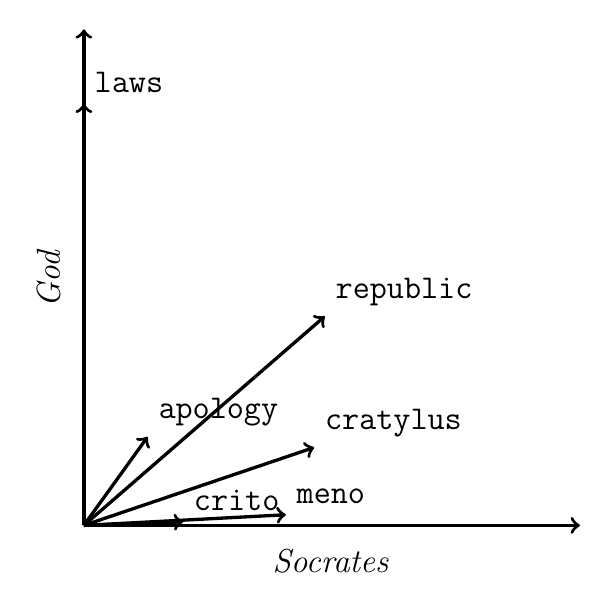
\begin{tikzpicture}[scale=0.45]
  \draw[->, very thick] (0,0) -- (14,0);
  \node at (7,-1) {\large{\emph{Socrates}}};
  \draw[->, very thick] (0,0) -- (0,14);
  \node at (-1,7) [rotate=90]{\large{\emph{God}}};
  \draw[->, very thick] (0,0) -- (0 , 11.9) node[above right]{\large{\texttt{laws}}};
  \draw[->, very thick] (0,0) -- (6.8 , 5.9) node[above right]{\large{\texttt{republic}}};
  \draw[->, very thick] (0,0) -- (6.5 , 2.2) node[above right]{\large{\texttt{cratylus}}};
  \draw[->, very thick] (0,0) -- (5.7 ,  0.3) node[above right]{\large{\texttt{meno}}};
  \draw[->, very thick] (0,0) -- (1.8 , 2.5) node[above right]{\large{\texttt{apology}}};
  \draw[->, very thick] (0,0) -- (2.8 ,  0.1) node[above right]{\large{\texttt{crito}}};
\end{tikzpicture}
\caption{Works of Plato arranged in a two dimensional term-space according to the number of times the terms ``God'' and ``Socrates'' occured in their tokenized forms.}\label{fig:plato-docs}
\end{center}
\end{figure}
The original purpose of these document-term matricies was to help relating the content of a document to queries about certain information. So, using our table above, if a query about Plato's writings contained the word ``God'' it would be more readily linked to \texttt{laws} and \texttt{apology}, wheras if the query contained ``Socrates'' the link would be with \texttt{crito} and \texttt{meno} instead.

\textcite{deerwester-1990-indexing-by-lsa} observed that this same procedure could be used to measure word-similarity, however ``a document is not necessarily the optimal length of text for measuring word similarity''. So the concept of a \emph{word-context} matrix is concieved.

\begin{definition}[Context window]
  given a token $w_i$ from a tokenized document $W_d$, the function $\operatorname{context}(w, b)$ returns a sequence containing the following and preceding $b$ tokens from $W_d$ not including $w_i$ itself. The variable $b$ is called the window size.
  \begin{equation}
    \operatorname{context}(w_i,b)=(w_{i-b},\,\dots,\,w_{i-1},\,w_{i+1},\,\dots,\,w_{i+b})
  \end{equation}
\end{definition}

\begin{example}[Context window]
  A context window around the word ``next'' in the quote \eqref{eq:virginia-context} with a window size of 3,
  \begin{align}
    &\texttt{\fbox{We\vphantom{hy}} \fbox{know\vphantom{hy}} \fbox{not\vphantom{hy}} \fbox{what\vphantom{hy}} \fbox{comes\vphantom{hy}} \fbox{next\vphantom{hy}}, \fbox{or\vphantom{hy}} \fbox{what\vphantom{hy}} \fbox{follows\vphantom{hy}} \fbox{after\vphantom{hy}}}. \quad-\text{{\sffamily\small Virginia Woolf}}\nonumber\\[-.5em]
    &\texttt{~~~~~~~~~~~~-3~~~~-2~~~~-1~~~~~0~~~~+1~~~~+2~~~~+3}\label{eq:virginia-context}
  \end{align}
  is given by the sequence:\vspace{-0.5em}
  \begin{equation*}
    \operatorname{context}\big(\;\fbox{\small{\texttt{next}\vphantom{hy}}}\;, 3\big)= (\;\fbox{\small{\texttt{not}\vphantom{hy}}}\;, \;\fbox{\small{\texttt{what}\vphantom{hy}}}\;, \;\fbox{\small{\texttt{comes}\vphantom{hy}}}\;, \;\fbox{\small{\texttt{or}\vphantom{hy}}}\;, \;\fbox{\small{\texttt{what}\vphantom{hy}}}\;, \;\fbox{\small{\texttt{follows}\vphantom{hy}}}\;)
  \end{equation*}
  \vspace{0.5em}
\end{example}

\begin{definition}[Word-context co-occurrence count]
  Given a tokenized document $W_d$, we denote the number of times a token $c$ appears in the context of another token $w^*$: $\#_c\;\operatorname{context}(w^*)$. Then, we denote the total number of times $c$ appears in the context of any instance of the $w^*$ token throught the document $W_d$ by
  \begin{equation}
    f(w^*,c,W_d)=\sum_{\{w\in d\;\mid\; w=w^*\}}\#_c\;\operatorname{context}(w)
  \end{equation}
  and, given a corpus of documents $C$ we denote the sum of all these co-occurrence counts over all the documents in the corpus:
  \begin{equation}
    F(w^*,c)=\sum_{d\in C}f(w^*,c)
  \end{equation}
\end{definition}

From here it is straightforward to define the word-context co-occurrence matrix:

\begin{definition}[Word-context co-occurrence matrix]
  Given a corpus of documents $C=d_1,d_2,\dots,d_n$, and a tokenizer $T$, a term document matrix $\bf{X}$ is given by:
  \begin{equation}
    \bf{X}=
  \begin{bmatrix}
    F(w_1,c_1) & F(w_1,c_2) & \dots  & F(w_1,c_m) \\
    F(w_2,c_1) & F(w_2,c_2) & \dots  & F(w_2,c_m) \\
    \vdots        & \vdots        & \ddots & \vdots          \\
    F(w_m,c_1) & F(w_m,c_2) & \dots  & F(w_m,c_m) \\
  \end{bmatrix}
  \end{equation}
  where the $w_i$ and $c_i$ terms are are both from the vocabulary of $C$, $V(C)=w_1,w_2,\dots,w_m=c_1,c_2,\dots,\c_m$.
  The number of times the $i^{\text{th}}$ word appears in a context window with the $j^{\text{th}}$ context word is then given by $\bf{X}_{ij}$.
\end{definition}

\begin{example}[Meno's answer]
  A word-context co-occurrence matrix generated using this procedure with a window size of 10, using the works of Plato as its corpus identified these words as the ten \emph{most similar} (using the cosine measeure of similarity) to ``virtue'':
  \begin{center}{\footnotesize
      \captionsetup{width=.91\linewidth}
      \begin{tabular}{c r r r r r r r r r r}
        \toprule
        word & \multicolumn{1}{c}{virtue} & \multicolumn{1}{c}{wisdom} & \multicolumn{1}{c}{a} & \multicolumn{1}{c}{justice} & \multicolumn{1}{c}{this} & \multicolumn{1}{c}{an} & \multicolumn{1}{c}{men} & \multicolumn{1}{c}{courage} & \multicolumn{1}{c}{knowledge} & \multicolumn{1}{c}{all} \\
        \midrule
        similarity & 0.999 & 0.981 & 0.980 & 0.978 & 0.977 & 0.976 & 0.972 & 0.972 & 0.972 & 0.972 \\
        \bottomrule
      \end{tabular}
      \captionof{table}{The most similar words to ``virtue'' according to a word-context matrix trained on the works of Plato.}\label{tab:plato-doc-term}
    }\end{center}
  clearly stopwords like ``a'' and ``this'' have been included because of their high frequency in all contexts -this problem is discussed in \autoref{sec:weighting}.
\end{example}

The consequence of using a particular one these two main co-occurrence matrix types (with documents as the basis elements or with context words as basis elements) corresponds the difference in semantic relatedness discussed in \autoref{sec:semantic-relatedness}. Words that notably co-occur in the context of a document are likely to be \emph{paradigmatic paralells}, whereas words which co-occur in the context of a window around a target word are likely to be \emph{semantically similar}. \textcite{sahlgreen-2006-the-word-space-model} explores this connection in more depth in his thesis.

\section{Weighting}\label{sec:weighting}
The problem with raw co-occurrence counts is, like we see in \autoref{tab:plato-doc-term}, that ``stop words'' like \emph{the}, which tell us very little about the meaning of a given passage, are the highest weighted elements wheras domain specific terms which are the most informative only occur infrequently so contribute less to the overall position of a count-based vector.

We remedy this by applying a weighting function to the elements of $\bf{X}$. ``The idea of weighting is to give more weight to surprising events and less weight to expected events'' \parencite{turney10-from-frequen-to-meanin}.

For document-term matricies the most commonly used weighting method is the ``term frequency $\times$ inverse document frequency'' approach. The idea is that a term's weight sould be high if it was frequent in that document, but rare in other documents. This formulation has two parts: the term frequency and the inverse document frequency. Both of these parts have a variety of forms, often justified heuristically but (\textcite{robertson-2004-understanding-idf} includes a good discussion of justifications for the method -concluding that the theory of relevance weights \parencite{robertson-1976-relevance-weighting} makes the strongest cast) nevertheless these methods ``have proved extraudinarily robust and ddifficult to beat, even by much more carefully worked out models and theories'' \parencite{robertson-2004-understanding-idf}.

\begin{definition}[Term frequency]
  The term frequency should be higher if the term is very frequent in the document and lower otherwise.
  Given a corpus $C$, a tokenizer $T$, and a co-occurrence count function $f$ such that $f(w,W_d)$ equals the number of times that a token $w$ appears in a tokenized document $W_d$, the term frequency $\times$ inverse document frequency weighting for $w$ \& $d$ is given by:
  \begin{align}
    \operatorname{tf}(w,W_d)=\frac{f(w,W_d)}{\sum_{t\in W_d}f(t,W_d)}
  \end{align}
\end{definition}

\begin{definition}[Inverse document frequency]
  The inverse document frequency captures the idea of a 'rare' word: it should be higher if the term appears only in very few documents, and lower if the term appears in the majority of documents. First we define the document frequency:

  Given a corpus $C$, a tokenizer $T$, and a token $t$, the document frequency $\operatorname{df}$ of the term $t$ is given by:
  \begin{equation}
    \operatorname{df}_{t,d}=\frac{\#\{d\in C\;\mid\;t\in W_d\}}{\#C}
  \end{equation}
  The ``inverse document frequency'' $\operatorname{idf}$ is then given by: $\operatorname{idf}_t=\frac{1}{\operatorname{df}_t}$. This raw frequency is commonly scaled with a $\log$ function. The heuristic justification for this is because the significance of a term does not increase in proportion to its frequency -we want to emphasise the less frequent and ``squash'' the weights of the more frequent. Finally this gives us:
  \begin{equation}
    \operatorname{idf}_t=\log\frac{1}{\operatorname{df}}
  \end{equation}
\end{definition}

\begin{definition}[TF-IDF weighting]
  The final weight is then given by combining these terms:
  \begin{equation}
    \operatorname{tfidf}_{t,d}=\operatorname{tf}_{t,d}\operatorname{idf}_t
  \end{equation}
\end{definition}

For word-context matricies the most common approach is to use a pointwise-mutual-information weighting (PMI).

The concept of pointwise mutual information (PMI) is defined in terms two jointly distributed random variables $X$ and $Y$. In the case of word-context matricies we are interested in the joint distribution of two tokens throughout the text corpus, $ww$, and $c$. We apply the concept of pointwise mutual information by approximating the joint distribution probabilites of $w$ and $c$.

\begin{definition}[PMI weighting]
  Recall that the formula for PMI is:
  \begin{equation*}
    I(w,c)=\log\frac{P(w,c)}{P(w)P(c)}
  \end{equation*}
  Given a corpus $C$, a tokenizer $T$, and a word-context co-occurrence count function $F$ such that $F(w,c)$ equals the number of times $w$ appeared with $c$ in its context, approximate the value of the terms $P(w,c), P(w), P(c)$ as with the terms $p_{w,c}, p_w, p_c$ defined as follows:
  \begin{align}
    p_{w,c}&=\frac{F(w,c)}{\sum_{s\in V(C)}\sum_{t\in V(C)}F(t,s)}\\[0.5em]
    p_{w}&=\frac{\sum_{t\in V(C)}F(w,t)}{\sum_{s\in V(C)}\sum_{t\in V(C)}F(t,s)}\\[0.5em]
    p_{c}&=\frac{\sum_{t\in V(T)}F(c,t)}{\sum_{s\in V(C)}\sum_{t\in V(C)}F(t,s)}
  \end{align}
  Then the PMI weight is defined:
  \begin{equation}
    \operatorname{pmi} (w, c)=\log\frac{1 + p_{w,c}}{p_w p_c}
  \end{equation}
  The $+1$ within the logarithm is to avoid evaluating the undefined $\log 0$ since often the numerator $(p_{w,c})$ is equal to zero because the tokens $w$ and $c$ never co-occurred.
\end{definition}

\section{Dimensionality Reduction}
One main issue with the word spaces produced by count models is they are inconveniently high dimensional (as many dimensions as there are word-types in the vocabulary), and that they are \emph{sparse}: a large number of the entries are zero.

One common approach to tackle this problem is to factor the sparse matrix into smaller dense matricies using a technique called \emph{singular value decomposition} (SVD) \parencite{dumais-1988-using-lsa-to-improve}. Another approach is \emph{feature selection} where only those terms considered informative beyond a certain threshold are included in the co-occurrence matrix and the rest are discarded.

\begin{figure}[H]
  \centering
  \captionsetup{width=.91\linewidth}
  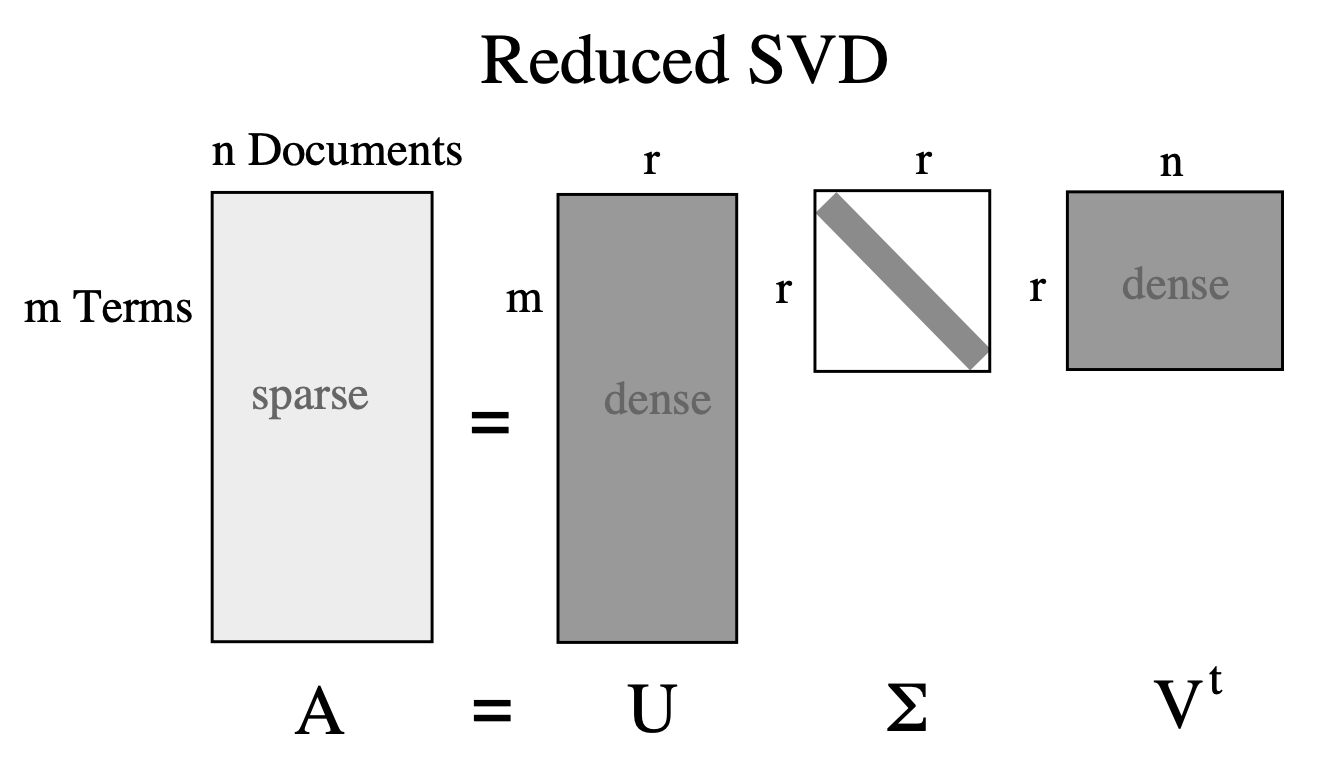
\includegraphics[scale=0.35]{figures/reduced-svd.png}
  \caption{Chart from \textcite{albright-2004-taming}. SVD decomposes $\bf{X}$ into three matricies: $\bf{U\sigma V}^T$. $\bf{U}$ and $\bf{V}$ are in column orthogonal form, and $\bf{\sigma}$ is a diagonal matrix of singular values. \parencite{golub13_matrix, turney10-from-frequen-to-meanin}}\label{fig:svd}
\end{figure}

\section{Comparison with other models}
Count models were the dominant approach to word embedding until \textcite{mikolov13-effic-estim-word-repres-vector-space} described a method for \emph{efficiently} generating embeddings using techniques from machine learning. Embeddings methods using machine learning techniques, called \emph{predict} models, initially developed somewhat independently. The first occurrence of this approach was in \parencite{bengio-2003-a-neural-prob-lang-model}, which described a machine-learning language model which produced word embeddings as a by-product of its primary function. Other predict models were concieved, improving upon this inital concept \parencite{morin-2005-hierarchical-probabilistic, mnih-2007-three-new-graphical-models, collobert-2008-a-unified-architecture} but this embedding paradigm remained less well known until until the success of \citeauthor{mikolov13-effic-estim-word-repres-vector-space}'s \parencite*{mikolov13-effic-estim-word-repres-vector-space} \texttt{word2vec} models encouraged direct comparisons and cross-paradigm research \parencite{baroni-etal-2014-dont, levy-2014-neural-WE-as}.

Although the methods seem quite different on the surface, \textcite{levy-2014-neural-WE-as} found that it is possible to view the operation of these predict models as \emph{implicitly} factoring a co-occurrence matrix -so theoretically the same information is being used by both models.

The methods we have presented here (document-term matricies and context-word matricies) are the foundation of the theory of count models but these particular models can vary greatly. Most notably, \citeauthor{pennington2014glove}'s \parencite*{pennington2014glove} GloVe model reports better results than other count-based models and prediction based models of the \texttt{word2vec} software package in the tasks of word-analogy and named entity recognition.

The cutting edge of embedding methods, at the time of writing is the ``deep contextualised model'' of \textcite{peters18-deep-contex-word-repres} which incorporates sentence-level information and leverages a language model to capture context-dependent aspects of word meaning. This is one particularly successful approach to tackling the difficulties endemic to word-meaning inference discussed in \nameref{chap:words} and \nameref{sec:semantic-relatedness}

%%% Local Variables:
%%% mode: latex
%%% TeX-master: "../main"
%%% End:
